% TODO units

Figure \ref{fig:system_design} illustrates our general system design approach
that simulates the ecovisor infrastructure and integrates it into the Mosaik
co-simulation environment while enabling SIL capabilities. The present design
can be categorized into two distinct parts, the simulation of the ecovisor, and
its interface to external applications, which are elaborated on in the
following.

\begin{figure}
    \centering
    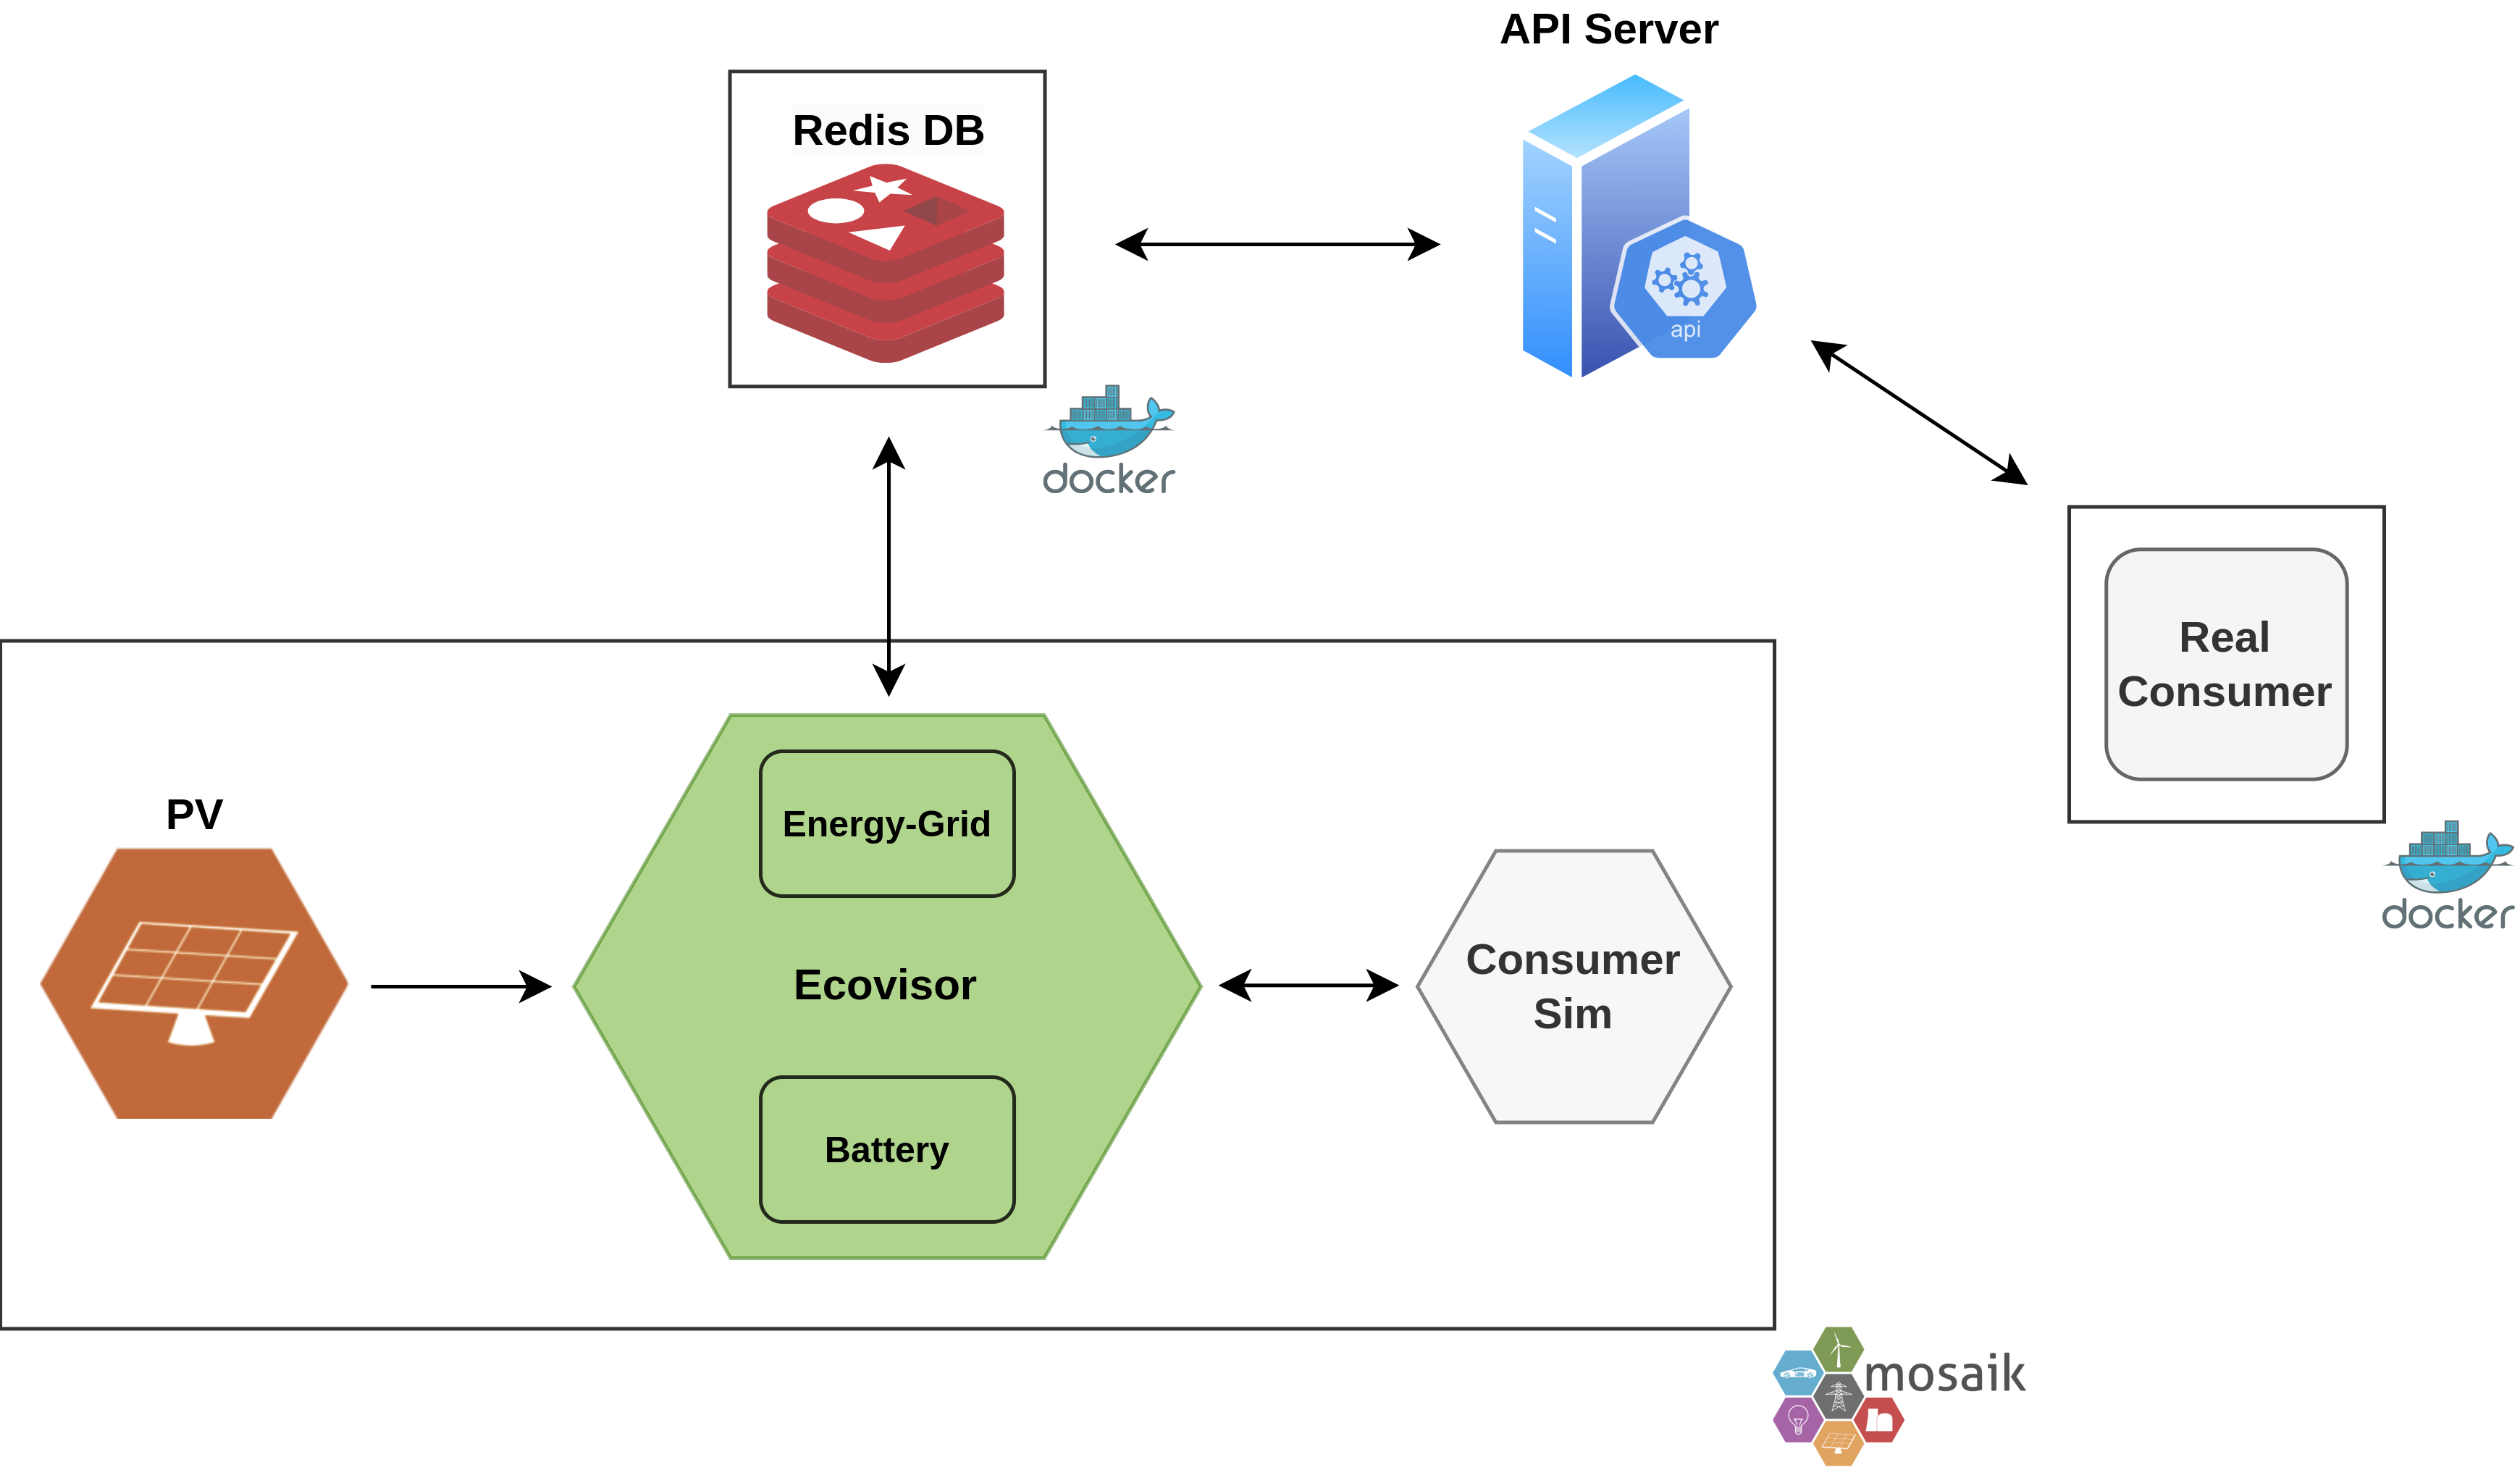
\includegraphics[width=\linewidth]{figures/system_design}
    \caption{
        General System Design: The ecovisor infrastructure is simulated and
        integrated into the Mosaik co-simulation environment. SIL capabilities
        are enabled via an API Server and a Redis database, connecting the
        simulation environment and real applications in real-time.
    }
    \label{fig:system_design}
\end{figure}

\subsection{Simulation of the Ecovisor}

\begin{figure}
    \removelatexerror
    \begin{algorithm}[H]
        \caption{Virtual Energy System Simulation}
        \label{alg:virtual_energy_system_simulation}
        $rest \gets consumption - solar$\;
        \eIf{$rest \leq 0$} {
            $b\_discharge\_rate \gets 0$\;
        }{
            $b\_discharge\_rate \gets \text{min}($\;
            \Indp
                $b\_max\_discharge,$\;
                $b\_charge\_level \cdot 3600,$\;
                $rest$\;
            \Indm
            $)$\;
            $rest \gets rest - b\_discharge\_rate$\;
        }
        $grid\_power \gets b\_charge\_rate + rest$\;
        $b.delta \gets b\_charge\_rate - b\_discharge\_rate$\;
        $b.step()$\;
        $b\_charge\_level \gets b.charge$\;
        $total\_carbon \gets grid\_carbon \cdot grid\_power$\;
        \vspace{3mm}
    \end{algorithm}
\end{figure}

\subsection{Interface to External Applications}

